\documentclass[a4paper,12pt]{article}

\usepackage{url}
\usepackage{epsfig}
\usepackage{graphics}
\usepackage{fancyhdr}

\graphicspath{{pictures/}}

\title{Report template for the project in the course DD2380 at KTH}
\author{\hspace*{-0.5cm}
GROUPXXXX\\
\begin{tabular}{cccc}
Author One & Author Two & Author Three & Author Four\\
BIRTHDATE1 & BIRTHDATE2 & BIRTHDATE3 & BIRTHDATE4 \\
MAIL1@kth.se & MAIL2@kth.se & MAIL3@kth.se & MAIL4@kth.se \\
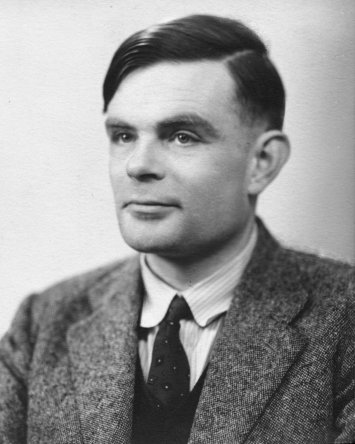
\includegraphics[width=0.13\linewidth]{Alan_Turing_photo} & 
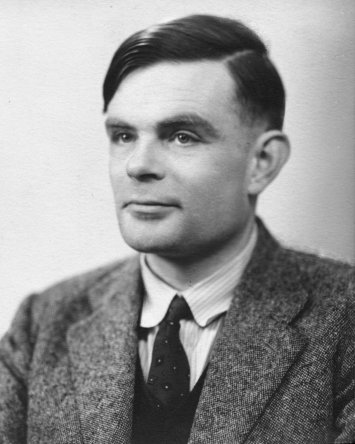
\includegraphics[width=0.13\linewidth]{Alan_Turing_photo} & 
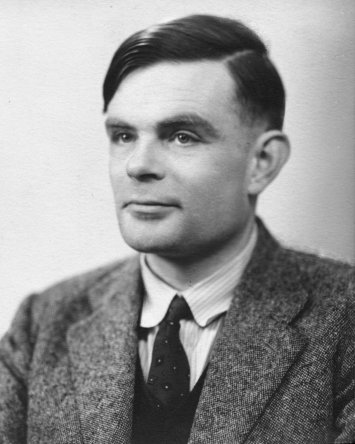
\includegraphics[width=0.13\linewidth]{Alan_Turing_photo} & 
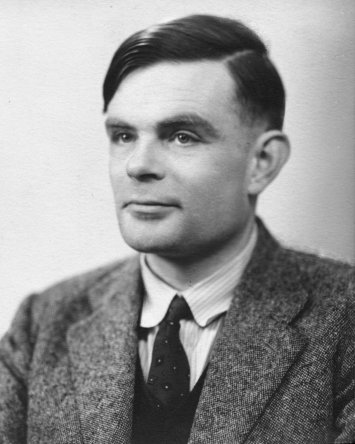
\includegraphics[width=0.13\linewidth]{Alan_Turing_photo}
\end{tabular}} 
% Normally there will not be any pictures but we want
% these so that we can connect faces to names in the course
% We also want birthdates so that we can tell people with the same
% name apart
\date{}

\pagestyle{fancy}
\setlength{\headheight}{15pt}
\fancyhf{}
\lhead{DD2380 ai14} % DO NOT REMOVE!!!!
\rhead{A. Andersson, S. Svensson} %% UPDATE WITH YOUR NAMES

\begin{document}

\maketitle
\thispagestyle{fancy}

\begin{abstract}
Bla bla bla bla bla bla bla bla bla bla bla bla bla bla bla bla bla 
bla bla bla bla bla bla bla bla bla bla bla bla bla bla bla bla bla 
bla bla bla bla bla bla bla bla bla bla bla bla bla bla bla bla bla 
bla bla bla bla bla bla bla bla bla bla bla bla bla bla bla bla bla
\end{abstract}



\clearpage

%%%%%%%%%%%%%%%%%%%%%%%%%%%%%%%%%%%%%%%%%%%%%%%%%%%%%%%%%%%%%
%%%%%%%%%%%%%%%%%%%%%%%%%%%%%%%%%%%%%%%%%%%%%%%%%%%%%%%%%%%%%
\section{Introduction (1--2 pages)}
\label{sec:intro}

Bla bla bla bla bla bla bla bla bla bla bla bla bla bla bla bla bla 
bla bla bla bla bla bla bla bla bla bla bla bla bla bla bla bla bla 
bla bla bla bla bla bla bla bla bla bla bla bla bla bla bla bla bla 
bla bla bla bla bla bla bla bla bla bla bla bla bla bla bla bla bla

\subsection{Contribution}

This project is done as an assignment in an introductory course in robotics and does not consist of any real contribution to the field of robotics. Most of the algorithms used in this report are simplifications of already well known and established algorithms. 
The report will however, hopefully be useful to any novice in the field seeking an insight into math and motion planning with multiple agents. 

\subsection{Outline}
Bla bla bla bla bla bla bla Section~\ref{sec:relwork} bla bla bla bla 
bla bla bla bla bla Section~\ref{sec:method} bla bla bla bla bla bla 
bla bla bla bla bla bla bla bla bla bla bla Section~\ref{sec:exps}
bla bla bla bla bla bla Section~\ref{sec:summary} bla bla bla bla bla

%%%%%%%%%%%%%%%%%%%%%%%%%%%%%%%%%%%%%%%%%%%%%%%%%%%%%%%%%%%%%
%%%%%%%%%%%%%%%%%%%%%%%%%%%%%%%%%%%%%%%%%%%%%%%%%%%%%%%%%%%%%
\section{Related work}
\label{sec:relwork}

Bla bla bla bla bla bla bla bla bla bla bla bla bla bla bla bla bla 
bla bla bla bla bla bla bla bla bla bla bla bla bla bla bla bla bla 
bla bla bla bla bla bla bla bla bla bla bla bla bla bla bla bla bla 
bla bla bla bla bla bla bla bla bla bla \cite{RussellNorvigAIBook3rd}
bla bla bla bla bla bla

%%%%%%%%%%%%%%%%%%%%%%%%%%%%%%%%%%%%%%%%%%%%%%%%%%%%%%%%%%%%%
%%%%%%%%%%%%%%%%%%%%%%%%%%%%%%%%%%%%%%%%%%%%%%%%%%%%%%%%%%%%%
\section{My method}
\label{sec:method}

The project consisted of three different parts: "Formation keeping", "Vehicle Routing Problem" and "Collision Avoidance".
In this section, each of these problems and the attempted solutions will be covered.

\subsection{"Formation Keeping"}
\label{sec:formation}

In this problem, the agents are placed in predetermined locations and need to enter a formation as fast as possible. Variations of this problem included:
A) Enter formation with global knowledge of the position of other agents.
B) Enter formation with local knowledge of the position of other agents.
C) Enter a moving formation.

The A) problem was solved by simply generating a greedy solution, which then was iteratively improved using an exhaustive search. The improvement process consisted of minimizing the sum of the cubes of the distances each agent had to traverse.
Meaning if vehicle A needed to traverse X meters and vehicle B Y meters, the expression that was minimized was X�+Y�. This heuristic panelizes the longer distances, and therefore results in a smaller Max distance across all agents.

The B) problem 

The C) problem   


\subsection{"Vehicle Routing Problem "}
\label{sec:vrp}

The "Vehicle Routing Problem"(VRP), is an NP problem similar to the "Travelling Salesman Problem"(TSP) problem. Unlike the TSP problem, where there is only one traveler traversing every city, we have multiple vehicles that need to divide the cities in between them. 

Our version of the VRP problem had some twists to it.
Firstly, we are minimizing time, and not distance. Secondly the movements our agents can perform are restricted by the agents motion model. 
This means that moving from one point to another is not a simple of traversing an Euclidean distance between the two points. Velocity, acceleration, direction and obstacles all play a major role in the path one would need to take when moving from A to B.

As with most NP problems, creating an algorithm that finds the optimal solution was not plausible. We therefore decided to look for an acceptable solution through the use of "Simulated Annealing".
For this approach, we needed a weighted graph of the map. This was created through the use of "Visibility Graphs" and "A*", using the length of the path created by A* as the weight of the edge. The Simulated Annealing algorithm would then create a greedy solution based on the graph, and make improvements using probabilistic methods.

However, we noticed this solution solved a much too simplified version of the problem at hand.  As explained earlier, the variable being minimized in this problem was time, not distance. Using Euclidean distances as weights in our graphs resulted in finding the shortest path that often could not be followed in a timely manner by a vehicle with restrictive motion models.

Generating accurate weights between each node was not possible due to the weight varying immensely on too many variables such as the ones described earlier. Instead we decided to use the simulated annealing algorithm, not to produce the shortest path, but to produce a large number of short paths. These paths could even be longer than the initial greedy path, as long as they were kept below a set threshold. 

We then would use "Rapidly exploring Random Tree"(RRT), to explore estimate the time it takes for the vehicle to traverse the path, and chose the one that resulted the shortest times.
Of course, this approach results in some additional margins of error, as RRT reacts extremely random. In order to minimize the effect of this additional randomness, we had to have our algorithm run repeatedly over longer periods of time.


\subsection{"Collision Avoidance "}
\label{sec:collision }

The Collision Avoidance problem during this project consisted of detection and avoiding not only obstacles, but also other vehicles with only local knowledge.

Our initial approach to solving the issue was to implement a repulsion mechanism to each agent. Whenever they get too close to an obstacle, or another agent, the agent would calculate the trajectory that would lead to a crash, and move in the exact opposite direction.
This however, lead to some weird behavior when cars in a collision course made symmetrical moves in order to avoid the collision, which then lead to a new collision course. The process would remind a lot of when 2 people try to get out of each other ways at the same time and end up blocking each other more.

The solution to this was to implement a priority order, where cars with higher priority ignore collision risks and the car with the lower priority work harder to try to avoid them. This did not completely work either, as sometimes, both cars need to take action in order for a collision to be avoided. 

A middle ground that worked well in the test cases was to have varying degrees of sensitivity amongst the cars. Where cars with low priority are way more sensitive and try to avoid collisions much earlier than a car with a higher priority, who will only start avoiding a collisions when its imminent.


%%%%%%%%%%%%%%%%%%%%%%%%%%%%%%%%%%%%%%%%%%%%%%%%%%%%%%%%%%%%%
%%%%%%%%%%%%%%%%%%%%%%%%%%%%%%%%%%%%%%%%%%%%%%%%%%%%%%%%%%%%%
\section{Experimental results}
\label{sec:exps}

Bla bla bla bla bla bla bla bla bla bla bla bla bla bla bla bla bla 
bla bla bla bla bla bla bla bla bla bla bla bla bla bla bla bla bla 
bla bla bla bla bla bla bla bla bla bla bla bla bla bla bla bla bla 

\subsection{Experiemntal setup}
Bla bla bla bla bla bla bla bla bla bla bla bla bla bla bla bla bla 
bla bla bla bla bla bla bla bla bla bla bla bla bla bla bla bla bla 
bla bla bla bla bla bla bla bla bla bla bla bla bla bla bla bla bla 

\subsection{Experiment ...}

Bla bla bla bla bla bla bla bla bla bla bla bla bla bla bla bla bla 
bla bla bla bla bla bla bla bla bla bla bla bla bla bla bla bla bla 
bla bla bla bla bla bla bla bla bla bla bla bla bla bla bla bla bla 

\begin{figure}
\centering
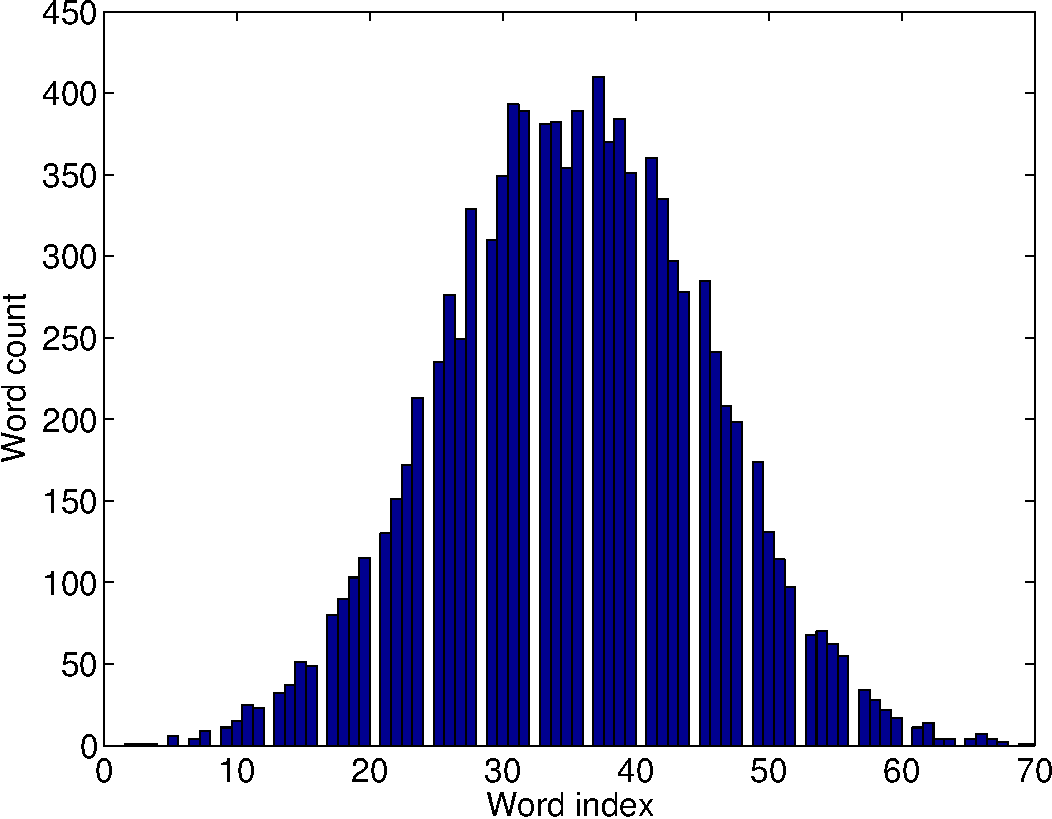
\includegraphics[width=0.8\linewidth]{histogram}
\caption{A description that makes browsing the paper easy and clearly 
describes what is in the picture. Make sure that the text in the figure 
is large enough to read and that the axes are labelled.}
\label{fig:histogram}
\end{figure}

Bla bla bla bla bla Figure~\ref{fig:histogram} bla bla bla bla bla bla 
bla bla bla bla bla bla bla bla bla bla bla bla bla bla bla bla bla 
bla bla bla bla bla bla bla bla bla bla bla bla bla bla bla bla bla 

\begin{table}
\begin{center}
\begin{tabular}{|c|c|c|}
\hline
Bla bla & Bla bla & Bla bla \\ \hline
42 & 42 & 42 \\ \hline
42 & 42 & 42 \\ \hline
\end{tabular}
\caption{A description that makes browsing the paper easy and clearly 
describes what is in the table.}
\label{tab:results}
\end{center}
\end{table}

Bla bla bla bla bla Table~\ref{tab:results} bla bla bla bla bla bla 
bla bla bla bla bla bla bla bla bla bla bla bla bla bla bla bla bla 
bla bla bla bla bla bla bla bla bla bla bla bla bla bla bla bla bla 

%%%%%%%%%%%%%%%%%%%%%%%%%%%%%%%%%%%%%%%%%%%%%%%%%%%%%%%%%%%%%
%%%%%%%%%%%%%%%%%%%%%%%%%%%%%%%%%%%%%%%%%%%%%%%%%%%%%%%%%%%%%
\section{Summary and Conclusions}
\label{sec:summary}

Bla bla bla bla bla bla bla bla bla bla bla bla bla bla bla bla bla 
bla bla bla bla bla bla bla bla bla bla bla bla bla bla bla bla bla 
bla bla bla bla bla bla bla bla bla bla bla bla bla bla bla bla bla 


%%%%%%%%%%%%%%%%%%%%%%%%%%%%%%%%%%%%%%%%%%%%%%%%%%%%%%%%%%%%%
%%%%%%%%%%%%%%%%%%%%%%%%%%%%%%%%%%%%%%%%%%%%%%%%%%%%%%%%%%%%%
\bibliographystyle{plain}
\bibliography{reflist}


\end{document}
